% (c) 2012 Dimitrios Vrettos - d.vrettos@gmail.com
% (c) 2017 Daniele Zambelli - daniele.zambelli@gmail.com
% 
% Tutti i grafici per il capitolo relativo ai razionali
% 
% 

% Colori per le divisioni:
\def \valposc{green!60!black} % Valore posizionale
\def \quozc{blue!60!black}    % Quoziente
\def \restc{red!60!black}     % Resto


\newcommand{\divisionea}{% divisione 4347:35
\begin{tikzpicture}
\tikzset{node distance=-25ex} 
\begin{scope}[font=\ttfamily]
\matrix (divisione) [matrix of nodes, ampersand replacement=\&]{%
  |[\valposc]|M\&|[\valposc]|C\&|[\valposc]|D\&|[\valposc]|U\\
  4 \& 3 \& 4 \& 7,\& 3 \& 5\\
    \& 8 \& 4 \&   \&
  |[\quozc]|1\&|[\quozc]|2\&|[\quozc]|4,\&|[\quozc]|2\&\\
    \& 1 \& 4 \& 7 \& 
  |[\valposc]|C\&|[\valposc]|D\&|[\valposc]|U\&|[\valposc]|d\\
    \&   \&   \& 7 \& 0\\
    \&   \&   \&   \& |[\restc]|0 \&\\
};
\end{scope}
\draw(divisione-2-5.north west)--(divisione-3-5.south west);
\draw(divisione-3-5.north west)--(divisione-3-8.north east);
\end{tikzpicture}
}

\newcommand{\divisioneb}{% divisione 1523:7
\begin{tikzpicture}
\tikzset{node distance=-25ex} 
\begin{scope}[font=\ttfamily]
\matrix (divisione) [matrix of nodes, ampersand replacement=\&]
{%
  |[\valposc]|M\&|[\valposc]|C\&|[\valposc]|D\&|[\valposc]|U\&
  |[\valposc]|d\&|[\valposc]|c\&|[\valposc] |m\\
  1 \& 5 \& 2 \& 3,\&   \&   \&   \& 7 \& ~ \& ~ \&\&\&\&\&\& ~ \&\\
    \& 1 \& 2 \&   \&   \&   \&   \&
|[\quozc]|2\&|[\quozc]|1\&|[\quozc]|7,\&|[\quozc]|5\&|[\quozc]|7\&
|[\quozc]| 1\&|[\quozc]|4\&|[\quozc]|6\&|[\quozc]|8\&   \&\\
    \&   \& 5 \& 3 \&   \&   \&   \& 
|[\valposc]|C\&|[\valposc]|D\&|[\valposc]|U\&|
[\valposc]|d\&|[\valposc]|c\&|[\valposc]|m\\
    \&   \&   \& 4 \& 0\\
    \&   \&   \&   \& 5 \& 0\\
    \&   \&   \&   \&   \& 1 \& 0\\
    \&   \&   \&   \&   \&   \& 3 \& 0\\
    \&   \&   \&   \&   \&   \&   \& 2 \& 0\\
    \&   \&   \&   \&   \&   \&   \&   \& 6 \& 0\\
    \&   \&   \&   \&   \&   \&   \&   \&   \& |[\restc]|4\\
};
\end{scope}
\draw(divisione-2-8.north west)--(divisione-3-8.south west);
\draw(divisione-2-8.south west)--(divisione-2-16.south east);
\end{tikzpicture}
}

\newcommand{\frazionea}{% parti della frazione
  \disegno{
    \node {$\dfrac{42}{75}$};
    \begin{scope}[\quozc]
    \draw [<-] (1, .5) to [out=0, in=180] (3, 2) node [right] 
      {~~~numeratore};
    \draw [->] (8.5, 2) to [out=0, in=180] (10.5, .5);
    \end{scope}
    \begin{scope}[\valposc]
    \draw [<-] (1, 0) -- (3, 0) node [right] {linea di frazione};
    \draw [->] (8.5, 0) -- (10.5, 0);
    \end{scope}
    \begin{scope}[red!50!black]
    \draw [<-] (1, -.5) to [out=0, in=180] (3, -2) node [right] 
      {~~denominatore};
    \draw [->] (8.5, -2) to [out=0, in=180] (10.5, -.5);
    \end{scope}
    \node at (11.5, 0) {$\dfrac{num}{den}$};
  }
}

\newcommand{\addizione}{% addizione algebrica tra frazioni
  \disegno{
    \node {$\dfrac{a}{b} \mp \dfrac{c}{d} \qquad = \qquad
             \dfrac{ad}{bd} \mp \dfrac{bc}{bd} = \dfrac{ad \mp bc}{bd}$};
    \begin{scope}[\quozc]
    \draw [->] (-5.5, 1) node [above right, yshift=3mm] {$\times d$} 
          to [out=45, in=135] (0, 1);
    \draw [->] (-5.5, -1) node [below right, yshift=-3mm] {$\times d$} 
          to [out=-45, in=-135] (0, -1);
    \end{scope}
    \begin{scope}[red!50!black]
    \draw [->] (-4, 1) to [out=45, in=135] (1.7, 1)
          node [above left, yshift=3mm] {$\times b$} ;
    \draw [->] (-4, -1) to [out=-45, in=-135] (1.7, -1)
          node [below left, yshift=-3mm] {$\times b$} ;
    \end{scope}
  }
}

\newcommand{\reciproco}{% reciproco di una frazione.
  \disegno{
    \node {$\dfrac{a}{b}$};
    \begin{scope}[\quozc]
    \path [postaction={decoration={text along path, text={reciproco},
           text align={align=center}}, decorate}] 
          (1, 0.2) to [out=45, in=180] (3, 0.8) to [out=0, in=135] (5, 0.2);
    \draw [<->] 
          (1, 0) to [out=45, in=180] (3, 0.6) to [out=0, in=135] (5, 0) 
;
    \end{scope}
    \node at (6, 0) {$\dfrac{b}{a}$};
  }
}

% \newcommand{\rettafra}[1]{% NON FUNZIONA, PERCHE'?
%   % Funzione rappresentata su due assi
%   \def \vals{#1}
%   \disegnod{10}{
%     \assecontrattini{-6}{+6}{0}{$\R$}
%     \foreach \x in {-6, ..., 5}{
%       \draw  (\x, 0) [below, font=\small] node {\x};
%     }
%     \foreach \x/\l in \vals{
%       \node at (\x, 0) [above] {\l};
%     }
%   }
% }

\newcommand{\rettafra}{% 
  % Frazioni rappresentate sull'asse
  \disegnod{10}{
    \assecontrattini{-6}{+6}{0}{\Q)}
    \foreach \x in {-6, ..., 5}{
      \draw  (\x, 0) [below, font=\small] node {\x};
    }
    \foreach \x/\l in {0.25 / $\frac{1}{4}$, 
                       0.5 / $\frac{1}{2}$, 
                       0.75 / $\frac{3}{4}$, 
                       1.33 / $\frac{4}{3}$,
                       1.66 / $\frac{5}{3}$,
                       2 / $\frac{6}{3}$,
                       2.5 / $\frac{5}{2}$, 
                       3.5 / $\frac{7}{2}$, 
                       4.8 / $\frac{24}{5}$,  
                       -1.33 / $-\frac{4}{3}$,
                       -2.5 / $-\frac{5}{2}$,
                       -3.66 / $-\frac{1}{3}$,
                       -4.5 / $-\frac{9}{2}$,
                       -5.66 / $-\frac{17}{3}$}{
      \draw [<-] (\x, 0) -- (\x, 0.3) node [above] {\l};
    }
  }
}

\newcommand{\frazdeca}{
\begin{tikzpicture}[node distance=-25ex]
  \begin{scope}[font=\ttfamily]
    \matrix (divisione) [matrix of nodes]
      {%
 1 & 9 & 7 & 8\\
   & 3 & 7 &|[blue]|2&|[blue]|~4,&|[blue]|6&|[blue]|2&|[blue]|5\\
   &   & 5 & 0\\
   &   &   & 2 & 0\\
   &   &   &   & 4 & 0\\
   &   &   &   &   & \(=\)\\
      };
  \end{scope}
  \draw (divisione-1-4.north west)--(divisione-2-4.south west);
  \draw (divisione-2-4.north west)--(divisione-2-8.north east);
  \node [left=of divisione-2-8.north west, yshift=-5mm] 
        {\(\dfrac{197}{8} = 28,625\)};
\end{tikzpicture}
}

\newcommand{\frazdecb}{

\begin{tikzpicture}[node distance=-25ex]
  \begin{scope}[font=\ttfamily]
    \matrix (divisione) [matrix of nodes]
      {%
 1 & 5 & 5 & 1 & 2\\
   & 3 & 5 &|[blue]|1&|[blue]|~2,&|[blue]|9&|[blue]|1&|[blue]|6\\
   & 1 & 1 & 0\\
   &   &   & 2 & 0\\
   &   &   &   & 8 & 0\\
   &   &   &   &   & 8\\
      };
  \end{scope}
  \draw(divisione-1-4.north west)--(divisione-2-4.south west);
  \draw(divisione-2-4.north west)--(divisione-2-8.north east);
  \node [left=of divisione-2-8.north west, yshift=-5mm] 
        {\(\dfrac{155}{12} = 12,91\overline{6}\)};
\end{tikzpicture}
}

\newcommand{\sottrazione}{

\begin{tikzpicture}[node distance=-25ex]
  \begin{scope}[font=\ttfamily]
    \matrix (divisione) [matrix of nodes]
      {%
\(1000n=\)& 1 & 4 & 3 & 5 & 6, & 5 & 6 & 5 & 6 & 5 & 6 & 5 & 6 & \dots 
&\(-\)\\
\(~~10n=\)&   &   & 1 & 4 & 3, & 5 & 6 & 5 & 6 & 5 & 6 & 5 & 6 & \dots 
&\(=\)\\
\(~990n=\)& 1 & 4 & 2 & 1 & 3, & 0 & 0 & 0 & 0 & 0 & 0 & 0 & 0 & \dots & ~\\
      };
  \end{scope}
  \draw(divisione-3-1.north west)--(divisione-2-16.south east);
\end{tikzpicture}
}

\newcommand{\horus}{
% (c) 2012 Dimitrios Vrettos - d.vrettos@gmail.com
% horus
% Occhio di Horus 
\pgfdeclareimage[interpolate=true]{eye}{\folder img/eye.png}
%{\folder img/eye.pdf}
\begin{tikzpicture}[scale=.7]
    \pgftext[at=\pgfpoint {0mm}{0mm},left,base]{\pgfuseimage{eye}}
    \node (a) at (10mm,65mm) {$\frac{1}{2}$};
    \node (b) at (30mm,65mm) {$\frac{1}{8}$};
    \node (c) at (50mm,65mm) {$\frac{1}{16}$};
    \node (d) at (10mm,0mm) {$\frac{1}{64}$};
    \node (e) at (30mm,0mm) {$\frac{1}{4}$};
    \node (f) at (50mm,0mm) {$\frac{1}{32}$};
  \begin{scope}[->,color=gray, thick]
    \draw (a)--(19mm,34mm);
    \draw (b)--(29mm,54mm);
    \draw (c)--(40mm,35mm);
    \draw (d)--(19mm,14mm);
    \draw (e)--(29mm,35mm);
    \draw (f)--(41mm,16mm);
  \end{scope}
\end{tikzpicture}
}

\newcommand{\frazioneb}{
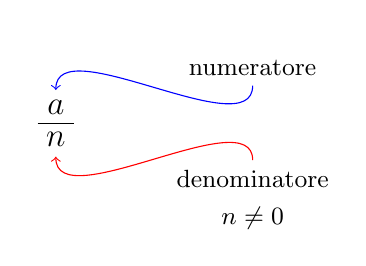
\begin{tikzpicture}
  \begin{scope}[font=\large]
    \matrix (frazione)  at (0,0){%
      \node (num) {$a$};\\
      \node (den) {$n$};\\
    };
  \end{scope}

  \draw (num.south west)--(num.south east);

  \begin{scope}[font=\small]
    \node (testo1) at (25mm,7mm) {numeratore};
    \node (testo2) at (25mm,-7mm) {denominatore};
    \node (testo3) at (25mm,-12mm) {$n\neq0$};
  \end{scope}

  \draw[->,blue] (testo1) .. controls +(down:10mm) and +(up:10mm) .. (num) ;
  \draw[->,red] (testo2) .. controls +(up:10mm) and +(down:10mm) .. (den) ;
\end{tikzpicture}
}

\newcommand{\rett}{
% (c) 2020 Daniele Zambelli
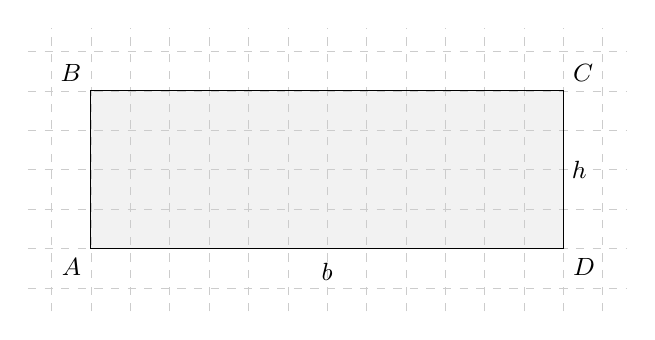
\begin{tikzpicture}[x=10mm,y=10mm,font=\small]

  \fill[fill=gray!10] (1,1) rectangle (7,3);
  \draw[style=help lines,step=5mm,dashed,black!20] (0.2,0.2) grid (7.8,3.8);
  \draw (1,1) rectangle (7,3);
  \node (b) at (4,.7) {$b$};
  \node (h) at (7.2,2) {$h$};
  \node [below left] at (1,1) {$A$};
  \node [above left] at (1,3) {$B$};
  \node [above right] at (7,3) {$C$};
  \node [below right] at (7,1) {$D$};

\end{tikzpicture}
}
